\chapter{Application to railway conflict management}

As a conclusion of the thesis, in this chapter we describe how the results presented so far can be
applied in the field of operational research. Namely, we propose an approach to solving the railway
dispatching problem using quantum annealing. We benchmark the implementation of our algorithm for
simple problem instances on the current generation of D-Wave annealers, using solutions obtained via
tensor networks and exhaustive search as a baseline for comparison.


\section{Overview of the problem}
Before formulating the problem to be solved, let us first introduce the necessary railway--related
terminology. We will consider a part of a railway network, which we will simply refer to as a
\emph{network}. The network is defined into \emph{block sections}. In our work, we focused only on
the single--track railways, and hence there are two possible kinds of sections:
\begin{itemize}
    \item Single tracks, sections that can be occupied by one train at a time.
    \item Sidings, or parallel tracks (occuring e.g. at stations). At the sidings, trains passing
      in the same direction can meet and overtake, and trains passing in the opposite directions
      can meet and pass. Each siding comprises two or more tracks, each of which can also be
      occupied by one train at a time.
\end{itemize}

Fig. \ref{fig:railway-network} shows an example network studied in our work. The trains move
through the network according to a \emph{timetable}. It is assumed that this timetable is conflict
free. That is, at any time no two trains occupy the same block section, except possibly at sidings
(where the number of trains does not exceed the number of tracks in the siding).

Now, suppose the network is affected by a disturbance, which prevented some trains from running
according to their original timetable. Put differently, after the disturbance, some trains occupy
different parts of the networks than they are supposed to occupy. Resuming operation according to
the original timetable could result in a conflict. Hence, after the disturbance, a new, conflict--free timetable has to be promptly created. Optimally, this new timetable should, in some sense, minimize the resulting delays.

It is important to distinguish two types of delays. A \emph{primary} delay is the one resulting
from the original disturbrance. There is some amount of time needed for a train to reach its
further destinations, e.g. due to speed limits and upper bound on speed achievable by a train.
Hence, primary delays propagate through the network and cannot be mitigated, even in the absence
of other trains. The delays resulting from the possible conflicts that need to be resolved are
called \emph{secondary} delays. The total delay is thus a sum of primary and secondary delays.
Since the primary delays are unavoidable, the objective is to minimize some function of secondary
delays, e.g. their maximum or weighted sum.

\begin{figure}
    \label{fig:railway-network}
    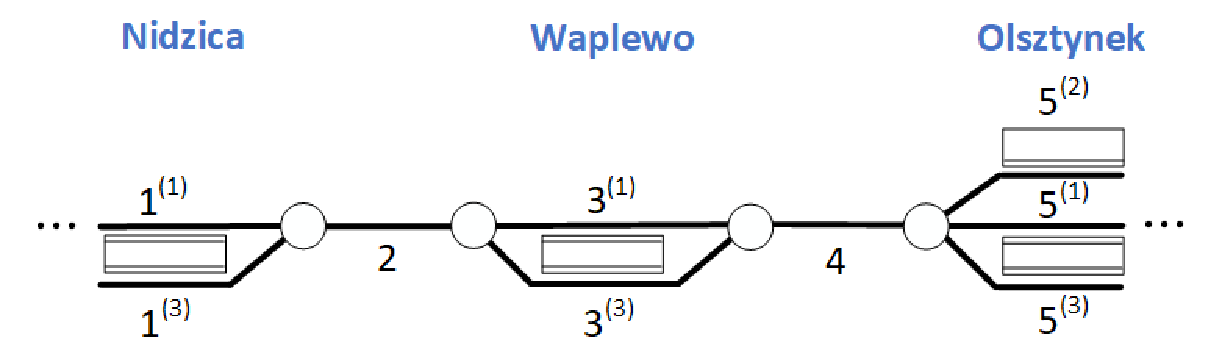
\includegraphics[width=\textwidth]{figures/line_small.pdf}
    \caption{
        Nidzica -- Olsztynek segment of line No. 216. Sections 1, 3, and 5 are parallel sidings,
        while sections 2 and 4 are single tracks.
    }
\end{figure}

\section{Basic defninition and notations}
Before we can formulate the optimization problem at hand in a way that it can be run on D-Wave,
let us introduce the needed notation. The set of all trains will be denoted by $\JJ$. This set is
naturally partitioned into the set $\JJ_0$ of trains going into one direction and set $\JJ_1$ of
trains going into the opposite direction. This is a proper partition, i.e.
\begin{equation}
    \JJ_0 \cup \JJ_1 = \JJ \quad \JJ_0 \cap \JJ_1 = \emptyset
\end{equation}

For any train $j \in \JJ$ its route $M_j$ is a sequence of blocks. Our model forbids recirculation,
 i.e. each train passes every block in its route exactly once, Furthermore, we assume that each
 train starts and ends its route at some station, and its route is uniquely identified by a
 sequence of station blocks
 $\left(s_{j,1}, s_{j, 2}, \ldots, s_{j, \mbox{end}_j}\right)$. In other words, there are no
 alternative routes between any two stations. For convenience, we will denote the block preceding
 $s_{j,k}$ in given train's route by $\pi(s_{j,k})$ and the block succeeding it by $\rho(s_{j,k})$,
 i.e.
 \begin{align}
     \pi(s_{j,k}) &= s_{j,k-1} \quad \mbox{for } 2 \le k \le \mbox{end}_j \\
     \rho(s_{j,k}) &= s_{j,k+1} \quad \mbox{for } 1 \le k \le \mbox{end}_j - 1.
 \end{align}

According to the original timetable, train $j$ should leave given station $s$ in its route at the time $\ttout(j, s)$. However, due to a disturbance a delay $d(j, s)$ can occur, in which case train
leaves at time $\tout = \ttout(j, s) + d(j, s)$. As already mentioned, primary delays propagate
through the network. However, they can be somewhat compensated if there is enough time reserved
in the passing sequence of blocks. Let us denote a primary delay of train $j$ at station $s$ as
$d_U(j, s)$. Then, the accumulated primary delay of the same train at the given station is
given by
\begin{equation}
    d_U(j, \rho(s)) = \max\{0, d_U(j, s) - \alpha(j, s, \rho(s))\}
\end{equation}
where $\alpha(j, s, \rho(s))$ accounts for possible time reserve.
\section{Formulating problem as quadratic binary optimization}


\section{Results}
In our work we considered two single-track railway lines managed by the polish state--owned company
PKP Polskie Linie Kolejowe:

\begin{itemize}
    \item Railway line No. 216 (Nidzica -- Olsztynek section)
    \item Railway line No. 191 (Goleszów -- Wisła -- Uzdrowisko section)
\end{itemize}
